\begin{multicols}{3}[\section{ZigBee}]

\rhead{Lucas Heuser, Simon Retzmann}
\lfoot{16.05.2016}

\newrefsegment

\begin{boxedminipage}{\linewidth}
\begin{tabular}{p{2,1 cm}p{2.7 cm}}
\textbf{Steckbrief}& \\
\end{tabular}
\rowcolors{1}{\topicolor!20}{}
\begin{tabular}{p{2,1 cm}p{2.7 cm}}
      Einsatz seit & 2004\\
      Frequenz"-bereich  & \SI{2,4}{\giga\hertz} (weltweit), \SI{868}{\mega\hertz} (Europa), \SI{915}{\mega\hertz} (USA)  \\				
      Datenrate & \SI{20}{kbit/s} - \SI{250}{kbit/s}\\
      Verbreitung & Weltweit, ZigBee-Allianz\\
      Reichweite & \SI{10}{\metre} - \SI{75}{\metre}\\
\end{tabular}
\end{boxedminipage}
\par
%Source http://www.fh-bingen.de/fileadmin/user_upload/Lehrende/Kilsch_Dieter/internet/projekte/TedoSchStiUnits.pdf -> Seite 9 findet ihr alle verwendbaren Einheiten, wie:
%\SI{Zahl}{\mega\hertz} oder \SI{Zahl}{\mili\metre}
%Ich weiß ehrlich gesagt nicht welche Einheiten ihr im Text genau braucht, aber in dem Dokument und mit obigen Beispiel sollte es umsetzbar ein.

\subsection*{Überblick}
Der Technologiestandard ZigBee ist ein weltweit offener Funkstandard, welcher von der ZigBee-Allianz entwickelt wurde. Ziel hierbei war es, einen einheitlichen Standard für Funknetzwerke mit Steuerungs- und Überwachungsaufgaben bereitstellen zu können.~\cite{zigbee.1} 
\begin{Figure}

\includegraphics[width=\linewidth]{Kapitel/ZigBee/Grafiken/zigbee_logo.png}
\captionof{figure}{ZigBee Logo~\cite{zigbee.8}}
\label{fig:vorlage.zemath}
\end{Figure}
Die Spezifikation wird vor allem im Bereich Hausautomation eingesetzt und wird sicherlich mit einer immer größer werdenden Verbreitung des Internet of Things eine stärkere Rolle im alltäglichen Umfeld einnehmen. 
ZigBee zeichnet sich durch eine hohe Ausfallsicherheit, eine umfangreiche und geräteübergreifende Kommunikation sowie geringem Energieverbrauch aus.~\cite{zigbee.2}

\subsection*{Technische Erläuterungen}
ZigBee ist ein für drahtlose Netzwerke entwickeltes Framework, zur Erstellung und Verwaltung von sogennanten ZigBee Netzwerken. Innerhalb dieser Netzwerke beschreibt der Standard wie unterschiedliche Geräte miteinander kommunizieren können und wie bestimmte Aktionen ausgeführt werden. Der Standard bietet ebenso Schnittstellen zu weiteren externen Netzen, wie dem Internet, um einzelne Geräte aus größerer Distanz fernsteuern zu können oder einzelne Daten abfragen zu können.
Die ZigBee Spezifikation ist eine Erweiterung des IEEE 802.15.4 Standards um eine Vermittlungs- und eine Anwendungsschicht (siehe Abbildung 2). 
\begin{Figure}
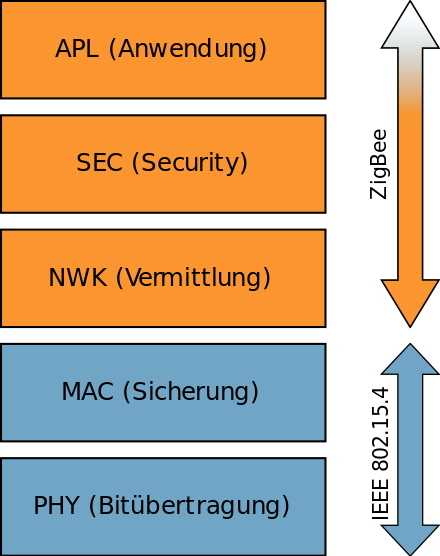
\includegraphics[width=\linewidth]{Kapitel/ZigBee/Grafiken/zigbee_stack.png}
\captionof{figure}{Einsatz des ZigBee Standards im OSI-Modell~\cite{zigbee.9}}
\label{fig:vorlage.zemath}
\end{Figure}
Die Vermittlungsschicht ist hierbei für das Routing und diverse Netzwerkfunktionen zuständig. Der Zugriff auf die direkt unterhalb liegende Sicherungsschicht und des hierbei eingesetzten Media Access Control (MAC) Protokolls erfolgt über sogenannte Dienstzugangspunkte/Service Access Points (SAPs).
\par Zu den Aufgaben von ZigBee innerhalb der Vermittlungsschicht zählen~\cite{zigbee.1}: 
\begin{itemize}
	\item Konfiguration von Funkmodulen
	\item Routing, Zustellung von Paketen
	\item Adresszuweisung
	\item Netzwerkmanagement, Verwaltung und Erstellung des ZigBee Netzwerkes
	\item Erstellung und Versenden von Netzwerkframes
\end{itemize}
Die in der ZigBee Spezifikation definierte Anwendungsschicht erhält ihre Daten ebenfalls über SAPs von der Vermittlungsschicht. Die Anwendungsschicht besteht aus folgenden drei Komponenten: 
\begin{itemize}
	\item Anwendungsunterstützungsschicht (APS)
	\item ZigBee Device Objekt (ZDO)
	\item Anwendungsframework
\end{itemize}
Hierbei dient das Anwendungsframework als eine Zusammenstellung aller im Netzwerk registrierten Anwendungsobjekte. Für jedes Objekt wird hierbei ein Identifikator (ID) zwischen 1 und 240 vergeben. Das ZDO übernimmt die Rolle des Anwendungsobjektes mit der ID 0 und hat die Aufgabe die APS und die zugehörige Vermittlungsschicht zu initialisieren. Die APS stellt die, durch die Anwendungsschicht geforderten Funktionen zur Verfügung und stellt diese der ZDO sowie den Anwendungsobjekten des Anwendungsframeworks bereit.~\cite{zigbee.1}
\subsubsection*{ZigBee Geräterollen}
Innerhalb der ZigBee Spezifikation wird zwischen drei verschiedenen Gerätetypen unterschieden, welche jeweils spezifische Rollen innerhalb des Netzwerkes erfüllen. Diese Gerätetypen sind: 
\begin{itemize}
	\item ZigBee End Device (ZED)
	\item ZigBee Router (ZR)
	\item ZigBee Coordinator (ZC)
\end{itemize}
Das ZED dient hierbei als, für den Benutzer direkt ersichtliches Gerät innerhalb des Netzwerkes. Hierzu zählen Endgeräte, welche zur Steuerung konkreter Aufgaben eingesetzt werden. Diese Geräte nehmen nicht am Routing des Netzwerkes teil und können bei Nichtverwendung in einen Ruhezustand versetzt werden. Die ZR dienen zum Routen der Informationspakete durch das Netzwerk. Jedes ZED kann hierbei ausschließlich mit einem Router kommunizieren. Die letzte Rolle innerhalb des Netzwerkes bildet der ZC, welcher zum initialen Aufbau des Netzwerkes benötigt werden. Nach dem Starten des Netzwerkes übernimmt der ZC die Rolle eines ZRs.~\cite{zigbee.10}

\subsection*{Einsatz}
Die Netzwerkspezifikation ZigBee findet vor allem im Bereich der Hausautomation Verwendung. Hier dient die Technologie dazu, verschiedene Systeme innerhalb eines Heimnetzwerkes miteinander zu koppeln und so untereinander kommunizieren zu lassen. Der Zugriff auf das interne Netzwerk soll ebenso von außerhalb ermöglicht werden. 
\par Die Vernetzung der einzelnen Geräte dient dazu, diese entweder automatisiert oder manuell ansprechen und steuern zu können. Ein Anwendungsfall hierfür wäre beispielsweise das Einschalten von Licht oder einem elektrischen Heizkörper per mobiler Applikation. Es ist ebenso möglich diverse Geräte innerhalb eines ZigBee Netzwerkes miteinander kommunizieren zu lassen und so einzelne Aufgaben verschiedener Geräte aufeinander abzustimmen. Dies ermöglicht, dass ein Auslösen eines Ereignis an einem einzelnen Gerät weitere Aktion anderer Geräten triggern kann. Eine denkbare Einsatzmöglichkeit wäre hier beispielsweise das Starten der Kaffeemaschine, nachdem der Alarm des Weckers ausgelöst wurde.  
\par Ein weiteres Anwendungsgebiet der Spezifikation ist im industriellen Bereich zu finden. Hier wird der ZigBee Standard im Bereich der Maschinenautomatisierung eingesetzt und dient dazu, bestimmte Daten auszulesen und zu übermitteln. So hilft ZigBee beispielsweise bei der Güterüberwachung, der Steuerung einzelner Anlagenelemente oder dem Übermitteln von Sensordaten an die nächste Produktionseinheit.~\cite{zigbee.10}

\subsection*{Anbieter und Gremien}
Gründer und offizieller Entwickler der ZigBee Spezifikation ist die sogenannte ZigBee-Allianz. Dieses Gremium ist ein globaler Zusammenschluss von Firmen, über Universitäten bis hin zu Einzelpersonen. Die einzelnen Mitglieder der Allianz sind unterteilt in die Kategorien Adopter, Participant und Promoter.


\end{multicols}
\newpage
\section*{Historische Entwicklung}
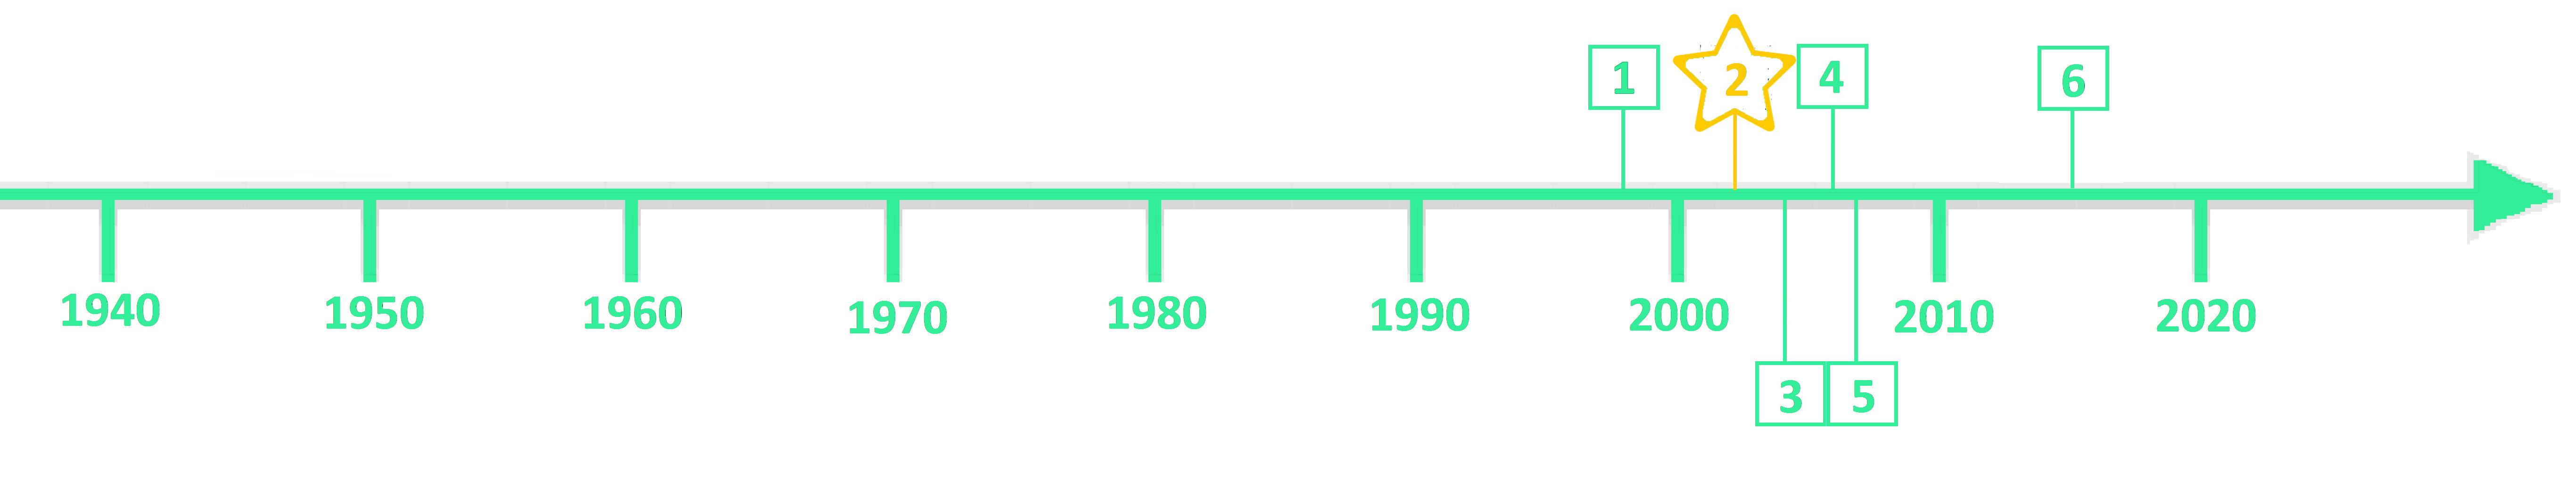
\includegraphics[width=\textwidth]{Kapitel/ZigBee/Grafiken/Zeitstrahl}
\par
\noindent
\rowcolors{2}{}{\topicolor!20}
\begin{tabular}{p{1 cm}p{3 cm}p{13.55 cm}}
	Nummer & Datum & Entwicklungsschritte~\cite{zigbee.5}\\
	1 & 1998 & Beginn der Entwicklung eines neuen Standards für kabellose Kommunikation zwischen Endgeräten mit geringen Datenraten.\\
	2 & 2002 & Gründung der ZigBee-Allianz.\\
	3 & 2004 & Veröffentlichung der ersten ZigBee Spezifikation.\\
	4 & 2006 & Veröffentlichung einer zweiten ZigBee Spezifikation.\\
	5 & 2007 & Einführung von ZigBee PRO, mit erweiterter Funktionalität.\\
	6 & 2015 & Auffinden einer gravierenden Sicherheitslücke, welche Angreifern den kompletten Zugriff auf ZigBee Geräte ermöglicht.\\
\end{tabular}
\par
\begin{multicols}{3}

%Dieser Kommentar ist vorerst zum Ignorieren gedacht. Er ist quasi gar nicht da. Hier wird kein Spaltenbreites Bild eingefügt. Nein. Wird es nicht.
%\end{multicols}
%\begin{FigureFullWidth}
%
\includegraphics[width=\textwidth, height = 0.125\textheight]{Kapitel/Vorlage/Grafiken/966a49a.jpg}
%\captionof{figure}{DHBW-Startseitenbild~\cite{vorlage.9}}
%\end{FigureFullWidth}
%\begin{multicols}{3}

Die einzelnen Kategorien unterscheiden sich in der Art und Weise, inwieweit bei Entwicklungsentscheidungen sowie Entscheidungen über organisatorische Angelegenheiten der Allianz mitbestimmt werden darf. Adopter, Participant und Promoter erhalten in aufsteigender Reihenfolge immer höhere Mitspracherechte. Allerdings steigen die Beiträge des Mitgliedes ebenso für jeden Kategorieanstieg.~\cite{zigbee.11} Weitere Details zu den genaueren Abstufungen und Beiträgen der einzelnen Kategorien sind auf der offiziellen ZigBee Webseite zu erfahren.
\par Da der ZigBee Standard als eine globale und offene Spezifikation entwickelt wurde, ist der Einsatz dieser Technologie in nahezu allen Endgeräten möglich. Von der ZigBee-Alliance  geprüfte Geräte werden allerdings mit einem Gütesiegel ausgestattet, um die korrekte Implementierung des Standards zu garantieren und somit die Kompatibilität zu anderen Geräten sicherzustellen. Ein Beispiel hierfür ist die HUE Serie von Philips, welche aus fernsteuerbaren LED-Lampen besteht.
\begin{Figure}
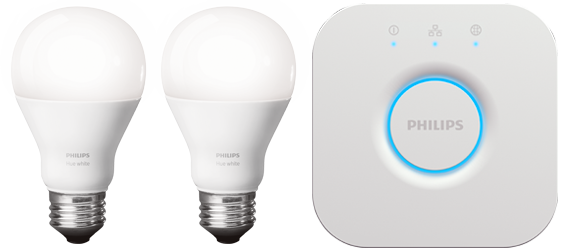
\includegraphics[width=\linewidth]{Kapitel/ZigBee/Grafiken/hue.png}
\captionof{figure}{Philips HUE Starter-Set, beispielhafter Anwendungsfall der ZigBee Spezifikation~\cite{zigbee.7}}
\label{fig:vorlage.zemath}
\end{Figure}

\subsection*{Historische Entwicklung und Sicherheitsrisiken}
Auf Grund der Erkenntnis, dass die Technologien Bluetooth und WiFi für gewisse Anwendungsfälle ungeeignet sind, wurde im Jahr 1998 an neuen Möglichkeiten zur Erstellung und Verwaltung von interaktiven Netzwerken geforscht. Diese Netzwerke sollten vor allem für die Kommunikation mit geringen Datenraten zwischen verschiedenen Endgeräten ausgelegt sein. 2002 wurde eine Allianz aus verschiedenen Unternehmen gegründet, welche sich der Entwicklung eines effizienten und effektiven Funkstandards, unter dem Namen ZigBee, als Ziel gesetzt hat. Die erste Version dieser Spezifikation kam im Jahre 2004 auf den Markt. Diese Version wurde 2006 von einer komplett überarbeiteten zweiten Version abgelöst. Ein Jahr später wurde eine Professional-Version der Spezifikation angeboten, welche über einen leicht erweiterten Funktionsumfang für Enterprise Kunden verfügt. 
Im Jahr 2015 wurde eine erhebliche Sicherheitslücke innerhalb der Spezifikation ausfindig gemacht, welche es Angreifern ermöglicht, die Kontrolle über einzelne Geräte eines ZigBee Netzwerkes zu übernehmen. Dieser Angriff ist möglich, weil es in der Spezifikation ein für die Verschlüsselung zuständiges Schlüsselpaar gibt, welches von jedem Gerät akzeptiert wird (Fallback Key) und öffentlich bekannt ist. Dieser Schlüssel wird verwendet um neue Geräte innerhalb eines Netzwerkes registrieren zu können. Nach der Regisistrierung wird ein spezifischer, nicht-öffentlicher Schlüssel verwendet. Wird nun allerdings ein neues Gerät im ZigBee Netzwerk vom Benutzer angemeldet, so fordert dieses neu hinzugefügte Gerät den nicht-öffentlichen symmetrischen Schlüssel an. Dieser wird nun zwar verschlüsselt an das neue Gerät gesendet, allerdings erfolgt die Verschlüsselung lediglich über den öffentlich bekannten Fallback Key. Liest nun ein Angreifer die erfolgte Funkkommunikation während des Anmeldevorgangs mit, so ist er in der Lage, den nicht-öffentlichen Schlüssel aus den Nachrichten herauszufiltern und mit Hilfe des Fallback Keys zu dekodieren.~\cite{zigbee.12} 

\subsection*{Ausblick}
Da sich ZigBee hauptsächlich mit dem Thema Smart Home und dem damit zusammenhängenden Thema Internet of Things auseinandersetzt und diese Themenbereiche in naher Zukunft wahrscheinlich immer größere Beachtung finden werden und somit auch in immer mehr Privathaushalten eingesetzt werden, ist ZigBee ein aktuelles und ebenso zukunftsorientiertes Thema. 
\par Auf Grund der erwähnten Sicherheitslücken in der aktuellen ZigBee Spezifikation, wird allerdings momentan geraten, betroffende Geräte nur in nicht sicherheitsrelevanten Bereichen des Hausumfeldes einzusetzen.~\cite{zigbee.6}
\par Es ist also abzuwarten, ob die Sicherheitsmängel behoben werden können und in wie fern sich die Spezifikation gegenüber direkten Konkurrenten, wie beispielsweise dem Kommunikationsstandard Z-Wave, auf dem freien Markt durchsetzen kann.  

\printbibliography[segment=14,heading=subbibliography]

\end{multicols}
\newpage
